% Options for packages loaded elsewhere
% Options for packages loaded elsewhere
\PassOptionsToPackage{unicode}{hyperref}
\PassOptionsToPackage{hyphens}{url}
\PassOptionsToPackage{dvipsnames,svgnames,x11names}{xcolor}
%
\documentclass[
  letterpaper,
  DIV=11,
  numbers=noendperiod]{scrartcl}
\usepackage{xcolor}
\usepackage{amsmath,amssymb}
\setcounter{secnumdepth}{-\maxdimen} % remove section numbering
\usepackage{iftex}
\ifPDFTeX
  \usepackage[T1]{fontenc}
  \usepackage[utf8]{inputenc}
  \usepackage{textcomp} % provide euro and other symbols
\else % if luatex or xetex
  \usepackage{unicode-math} % this also loads fontspec
  \defaultfontfeatures{Scale=MatchLowercase}
  \defaultfontfeatures[\rmfamily]{Ligatures=TeX,Scale=1}
\fi
\usepackage{lmodern}
\ifPDFTeX\else
  % xetex/luatex font selection
\fi
% Use upquote if available, for straight quotes in verbatim environments
\IfFileExists{upquote.sty}{\usepackage{upquote}}{}
\IfFileExists{microtype.sty}{% use microtype if available
  \usepackage[]{microtype}
  \UseMicrotypeSet[protrusion]{basicmath} % disable protrusion for tt fonts
}{}
\makeatletter
\@ifundefined{KOMAClassName}{% if non-KOMA class
  \IfFileExists{parskip.sty}{%
    \usepackage{parskip}
  }{% else
    \setlength{\parindent}{0pt}
    \setlength{\parskip}{6pt plus 2pt minus 1pt}}
}{% if KOMA class
  \KOMAoptions{parskip=half}}
\makeatother
% Make \paragraph and \subparagraph free-standing
\makeatletter
\ifx\paragraph\undefined\else
  \let\oldparagraph\paragraph
  \renewcommand{\paragraph}{
    \@ifstar
      \xxxParagraphStar
      \xxxParagraphNoStar
  }
  \newcommand{\xxxParagraphStar}[1]{\oldparagraph*{#1}\mbox{}}
  \newcommand{\xxxParagraphNoStar}[1]{\oldparagraph{#1}\mbox{}}
\fi
\ifx\subparagraph\undefined\else
  \let\oldsubparagraph\subparagraph
  \renewcommand{\subparagraph}{
    \@ifstar
      \xxxSubParagraphStar
      \xxxSubParagraphNoStar
  }
  \newcommand{\xxxSubParagraphStar}[1]{\oldsubparagraph*{#1}\mbox{}}
  \newcommand{\xxxSubParagraphNoStar}[1]{\oldsubparagraph{#1}\mbox{}}
\fi
\makeatother

\usepackage{color}
\usepackage{fancyvrb}
\newcommand{\VerbBar}{|}
\newcommand{\VERB}{\Verb[commandchars=\\\{\}]}
\DefineVerbatimEnvironment{Highlighting}{Verbatim}{commandchars=\\\{\}}
% Add ',fontsize=\small' for more characters per line
\usepackage{framed}
\definecolor{shadecolor}{RGB}{241,243,245}
\newenvironment{Shaded}{\begin{snugshade}}{\end{snugshade}}
\newcommand{\AlertTok}[1]{\textcolor[rgb]{0.68,0.00,0.00}{#1}}
\newcommand{\AnnotationTok}[1]{\textcolor[rgb]{0.37,0.37,0.37}{#1}}
\newcommand{\AttributeTok}[1]{\textcolor[rgb]{0.40,0.45,0.13}{#1}}
\newcommand{\BaseNTok}[1]{\textcolor[rgb]{0.68,0.00,0.00}{#1}}
\newcommand{\BuiltInTok}[1]{\textcolor[rgb]{0.00,0.23,0.31}{#1}}
\newcommand{\CharTok}[1]{\textcolor[rgb]{0.13,0.47,0.30}{#1}}
\newcommand{\CommentTok}[1]{\textcolor[rgb]{0.37,0.37,0.37}{#1}}
\newcommand{\CommentVarTok}[1]{\textcolor[rgb]{0.37,0.37,0.37}{\textit{#1}}}
\newcommand{\ConstantTok}[1]{\textcolor[rgb]{0.56,0.35,0.01}{#1}}
\newcommand{\ControlFlowTok}[1]{\textcolor[rgb]{0.00,0.23,0.31}{\textbf{#1}}}
\newcommand{\DataTypeTok}[1]{\textcolor[rgb]{0.68,0.00,0.00}{#1}}
\newcommand{\DecValTok}[1]{\textcolor[rgb]{0.68,0.00,0.00}{#1}}
\newcommand{\DocumentationTok}[1]{\textcolor[rgb]{0.37,0.37,0.37}{\textit{#1}}}
\newcommand{\ErrorTok}[1]{\textcolor[rgb]{0.68,0.00,0.00}{#1}}
\newcommand{\ExtensionTok}[1]{\textcolor[rgb]{0.00,0.23,0.31}{#1}}
\newcommand{\FloatTok}[1]{\textcolor[rgb]{0.68,0.00,0.00}{#1}}
\newcommand{\FunctionTok}[1]{\textcolor[rgb]{0.28,0.35,0.67}{#1}}
\newcommand{\ImportTok}[1]{\textcolor[rgb]{0.00,0.46,0.62}{#1}}
\newcommand{\InformationTok}[1]{\textcolor[rgb]{0.37,0.37,0.37}{#1}}
\newcommand{\KeywordTok}[1]{\textcolor[rgb]{0.00,0.23,0.31}{\textbf{#1}}}
\newcommand{\NormalTok}[1]{\textcolor[rgb]{0.00,0.23,0.31}{#1}}
\newcommand{\OperatorTok}[1]{\textcolor[rgb]{0.37,0.37,0.37}{#1}}
\newcommand{\OtherTok}[1]{\textcolor[rgb]{0.00,0.23,0.31}{#1}}
\newcommand{\PreprocessorTok}[1]{\textcolor[rgb]{0.68,0.00,0.00}{#1}}
\newcommand{\RegionMarkerTok}[1]{\textcolor[rgb]{0.00,0.23,0.31}{#1}}
\newcommand{\SpecialCharTok}[1]{\textcolor[rgb]{0.37,0.37,0.37}{#1}}
\newcommand{\SpecialStringTok}[1]{\textcolor[rgb]{0.13,0.47,0.30}{#1}}
\newcommand{\StringTok}[1]{\textcolor[rgb]{0.13,0.47,0.30}{#1}}
\newcommand{\VariableTok}[1]{\textcolor[rgb]{0.07,0.07,0.07}{#1}}
\newcommand{\VerbatimStringTok}[1]{\textcolor[rgb]{0.13,0.47,0.30}{#1}}
\newcommand{\WarningTok}[1]{\textcolor[rgb]{0.37,0.37,0.37}{\textit{#1}}}

\usepackage{longtable,booktabs,array}
\newcounter{none} % for unnumbered tables
\usepackage{calc} % for calculating minipage widths
% Correct order of tables after \paragraph or \subparagraph
\usepackage{etoolbox}
\makeatletter
\patchcmd\longtable{\par}{\if@noskipsec\mbox{}\fi\par}{}{}
\makeatother
% Allow footnotes in longtable head/foot
\IfFileExists{footnotehyper.sty}{\usepackage{footnotehyper}}{\usepackage{footnote}}
\makesavenoteenv{longtable}
\usepackage{graphicx}
\makeatletter
\newsavebox\pandoc@box
\newcommand*\pandocbounded[1]{% scales image to fit in text height/width
  \sbox\pandoc@box{#1}%
  \Gscale@div\@tempa{\textheight}{\dimexpr\ht\pandoc@box+\dp\pandoc@box\relax}%
  \Gscale@div\@tempb{\linewidth}{\wd\pandoc@box}%
  \ifdim\@tempb\p@<\@tempa\p@\let\@tempa\@tempb\fi% select the smaller of both
  \ifdim\@tempa\p@<\p@\scalebox{\@tempa}{\usebox\pandoc@box}%
  \else\usebox{\pandoc@box}%
  \fi%
}
% Set default figure placement to htbp
\def\fps@figure{htbp}
\makeatother





\setlength{\emergencystretch}{3em} % prevent overfull lines

\providecommand{\tightlist}{%
  \setlength{\itemsep}{0pt}\setlength{\parskip}{0pt}}



 


\usepackage{fvextra}
\DefineVerbatimEnvironment{Highlighting}{Verbatim}{breaklines,commandchars=\\\{\}}
\KOMAoption{captions}{tableheading}
\makeatletter
\@ifpackageloaded{caption}{}{\usepackage{caption}}
\AtBeginDocument{%
\ifdefined\contentsname
  \renewcommand*\contentsname{Table of contents}
\else
  \newcommand\contentsname{Table of contents}
\fi
\ifdefined\listfigurename
  \renewcommand*\listfigurename{List of Figures}
\else
  \newcommand\listfigurename{List of Figures}
\fi
\ifdefined\listtablename
  \renewcommand*\listtablename{List of Tables}
\else
  \newcommand\listtablename{List of Tables}
\fi
\ifdefined\figurename
  \renewcommand*\figurename{Figure}
\else
  \newcommand\figurename{Figure}
\fi
\ifdefined\tablename
  \renewcommand*\tablename{Table}
\else
  \newcommand\tablename{Table}
\fi
}
\@ifpackageloaded{float}{}{\usepackage{float}}
\floatstyle{ruled}
\@ifundefined{c@chapter}{\newfloat{codelisting}{h}{lop}}{\newfloat{codelisting}{h}{lop}[chapter]}
\floatname{codelisting}{Listing}
\newcommand*\listoflistings{\listof{codelisting}{List of Listings}}
\makeatother
\makeatletter
\makeatother
\makeatletter
\@ifpackageloaded{caption}{}{\usepackage{caption}}
\@ifpackageloaded{subcaption}{}{\usepackage{subcaption}}
\makeatother
\usepackage{bookmark}
\IfFileExists{xurl.sty}{\usepackage{xurl}}{} % add URL line breaks if available
\urlstyle{same}
\hypersetup{
  pdftitle={ENVS 193DS Homework 3},
  pdfauthor={Steven Le},
  colorlinks=true,
  linkcolor={blue},
  filecolor={Maroon},
  citecolor={Blue},
  urlcolor={Blue},
  pdfcreator={LaTeX via pandoc}}


\title{ENVS 193DS Homework 3}
\author{Steven Le}
\date{2026-05-23}
\begin{document}
\maketitle


\section{Homework set up}\label{homework-set-up}

\begin{Shaded}
\begin{Highlighting}[]
\CommentTok{\#read in packages}
\FunctionTok{library}\NormalTok{(tidyverse)}
\FunctionTok{library}\NormalTok{(here)}
\FunctionTok{library}\NormalTok{(janitor)}
\FunctionTok{library}\NormalTok{(readxl)}
\FunctionTok{library}\NormalTok{(ggplot2)}
\FunctionTok{library}\NormalTok{(ggeffects)}
\FunctionTok{library}\NormalTok{(flextable)}
\FunctionTok{library}\NormalTok{(here)}
\CommentTok{\#stored kelp data as an object called kelp}
\NormalTok{kelp }\OtherTok{\textless{}{-}} \FunctionTok{read\_csv}\NormalTok{(}\FunctionTok{here}\NormalTok{(}\StringTok{"data"}\NormalTok{, }\StringTok{"temp{-}kelp.csv"}\NormalTok{))}
\CommentTok{\#stored personal data as an object called personal}
\NormalTok{personal }\OtherTok{\textless{}{-}} \FunctionTok{read\_csv}\NormalTok{(}\FunctionTok{here}\NormalTok{(}\StringTok{"data"}\NormalTok{, }\StringTok{"personal\_data.csv"}\NormalTok{))}
\end{Highlighting}
\end{Shaded}

\section{Problem 1. Giant kelp
fronds}\label{problem-1.-giant-kelp-fronds}

\subsection{a.}\label{a.}

To determine the strength of the relationship between temperature and
giant kelp frond elongation, you need to conduct a Pearson's correlation
test and Spearman rank correlation test. A Pearson's correlation test is
a parametric test that analyzes a linear relationship between continuous
variables that are normally distributed (debatable). On the other hand,
a Spearman rank correlation test is the non-parametric version that
looks as a monotonic relationship between variables that have
independently observed samples.

\subsection{b.}\label{b.}

\begin{Shaded}
\begin{Highlighting}[]
\CommentTok{\#base layer: ggplot}
\FunctionTok{ggplot}\NormalTok{(}\AttributeTok{data =}\NormalTok{ kelp,}
\CommentTok{\#x{-}axis: temperature, y{-}axis: kelp elongation rate       }
       \AttributeTok{mapping =} \FunctionTok{aes}\NormalTok{(}\AttributeTok{x =}\NormalTok{ temp\_c,}
                     \AttributeTok{y =}\NormalTok{ kelp\_elong)) }\SpecialCharTok{+} 
\CommentTok{\#first layer: geom\_point}
  \FunctionTok{geom\_point}\NormalTok{(}\AttributeTok{color =} \StringTok{"darkgreen"}\NormalTok{) }\SpecialCharTok{+} \CommentTok{\#changed color of points to dark green}
\CommentTok{\#renamed x{-} and y{-}axes and added units  }
  \FunctionTok{labs}\NormalTok{(}\AttributeTok{x =} \StringTok{"Temperature (\textbackslash{}u00B0C)"}\NormalTok{,}
       \AttributeTok{y =} \StringTok{"Kelp Elongation Rate (cm/day)"}\NormalTok{) }\SpecialCharTok{+}
\CommentTok{\#changed theme from default  }
  \FunctionTok{theme\_minimal}\NormalTok{()}
\end{Highlighting}
\end{Shaded}

\pandocbounded{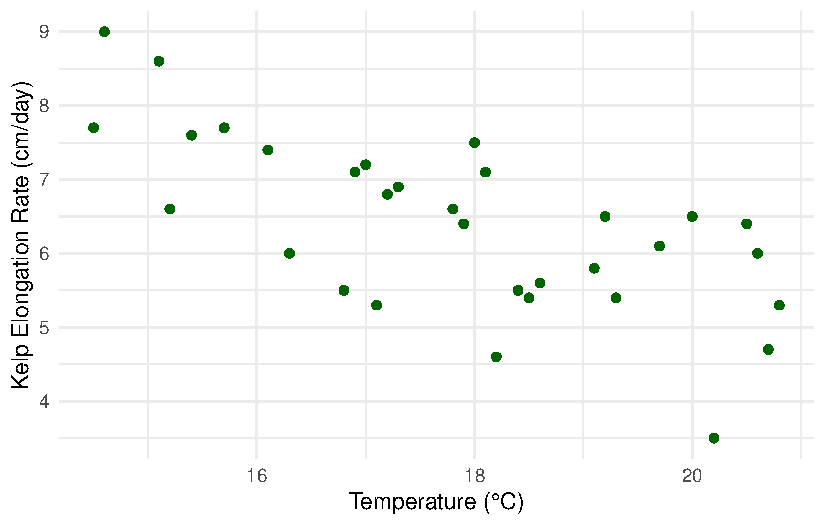
\includegraphics[keepaspectratio]{homework-3_files/figure-pdf/unnamed-chunk-2-1.pdf}}

\subsection{c.}\label{c.}

\subsection{QQ plot figure for
temperature:}\label{qq-plot-figure-for-temperature}

\begin{Shaded}
\begin{Highlighting}[]
\CommentTok{\#base layer: ggplot with starting data frame}
\FunctionTok{ggplot}\NormalTok{(}\AttributeTok{data =}\NormalTok{ kelp,}
\CommentTok{\#y{-}axis for QQ plot (no x{-}axis)}
\FunctionTok{aes}\NormalTok{(}\AttributeTok{sample =}\NormalTok{ temp\_c)) }\SpecialCharTok{+}
\CommentTok{\#first layer: QQ reference line colored red}
\FunctionTok{geom\_qq\_line}\NormalTok{(}\AttributeTok{color =} \StringTok{"red"}\NormalTok{) }\SpecialCharTok{+}
\CommentTok{\#second layer: QQ plot}
\FunctionTok{geom\_qq}\NormalTok{() }
\end{Highlighting}
\end{Shaded}

\pandocbounded{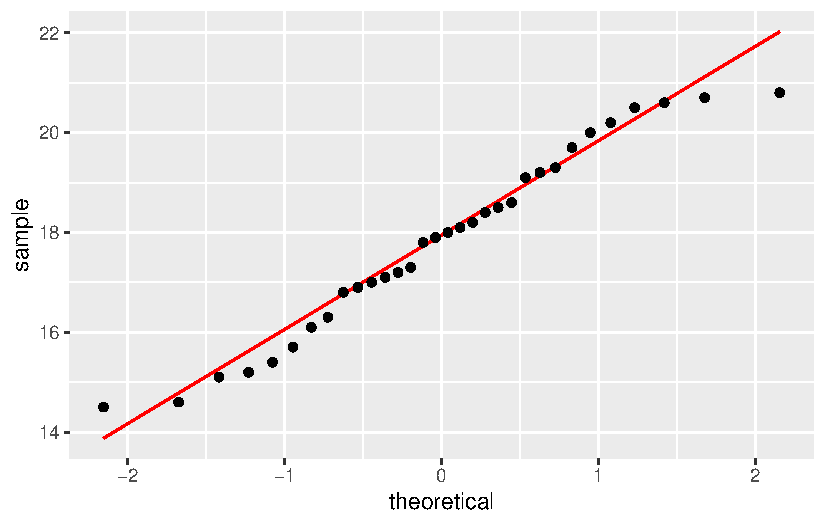
\includegraphics[keepaspectratio]{homework-3_files/figure-pdf/unnamed-chunk-3-1.pdf}}

\subsection{QQ plot figure for giant kelp frond elongation
rate:}\label{qq-plot-figure-for-giant-kelp-frond-elongation-rate}

\begin{Shaded}
\begin{Highlighting}[]
\CommentTok{\#base layer: ggplot with starting data frame}
\FunctionTok{ggplot}\NormalTok{(}\AttributeTok{data =}\NormalTok{ kelp,}
\CommentTok{\#y{-}axis for QQ plot (no x{-}axis)}
\FunctionTok{aes}\NormalTok{(}\AttributeTok{sample =}\NormalTok{ kelp\_elong)) }\SpecialCharTok{+}
\CommentTok{\#first layer: QQ reference line colored red}
\FunctionTok{geom\_qq\_line}\NormalTok{(}\AttributeTok{color =} \StringTok{"red"}\NormalTok{) }\SpecialCharTok{+}
\CommentTok{\#second layer: QQ plot}
\FunctionTok{geom\_qq}\NormalTok{() }
\end{Highlighting}
\end{Shaded}

\pandocbounded{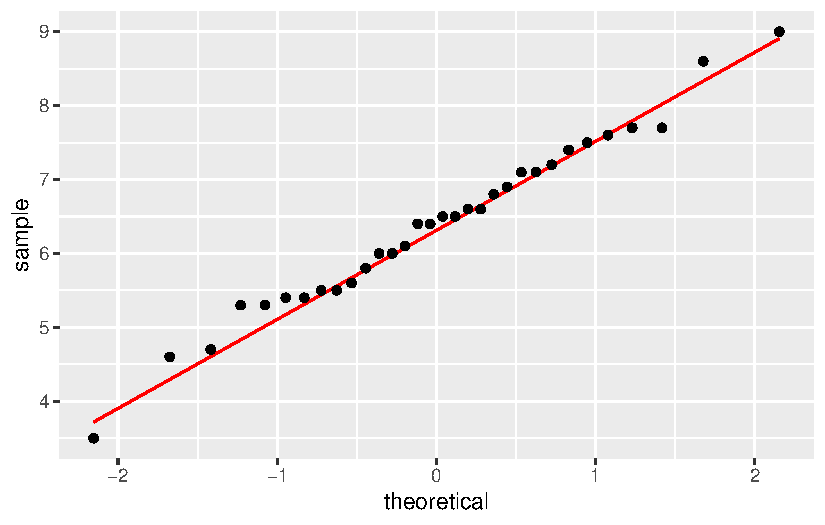
\includegraphics[keepaspectratio]{homework-3_files/figure-pdf/unnamed-chunk-4-1.pdf}}

\subsection{Evaluating Pearson's correlation test
assumptions:}\label{evaluating-pearsons-correlation-test-assumptions}

By making QQ plots for each of the two variables, we were able to
interpret if the variables, respectively, are normally distributed.
Looking at both QQ plots, temperature (Celsius) and giant kelp frond
elongation rate (cm/day) look normally distributed as most of the points
roughly follow the reference line in each plot. For the other three
assumptions, there does seem to be a linear (negative) relationship
between the variables based on the scatterplot, the variables are
definitely continuous, and we can give the benefit of the doubt that the
data were collected through independent observations.

\subsection{Pearson's correlation test code
chunk:}\label{pearsons-correlation-test-code-chunk}

\begin{Shaded}
\begin{Highlighting}[]
\CommentTok{\#ran a correlation test between temperature and kelp elongation rate}
\FunctionTok{cor.test}\NormalTok{(kelp}\SpecialCharTok{$}\NormalTok{kelp\_elong, kelp}\SpecialCharTok{$}\NormalTok{temp\_c,}
\CommentTok{\#used Pearson\textquotesingle{}s r correlation test as our method         }
         \AttributeTok{method =} \StringTok{"pearson"}\NormalTok{)}
\end{Highlighting}
\end{Shaded}

\begin{verbatim}

    Pearson's product-moment correlation

data:  kelp$kelp_elong and kelp$temp_c
t = -5.189, df = 30, p-value = 1.366e-05
alternative hypothesis: true correlation is not equal to 0
95 percent confidence interval:
 -0.8359665 -0.4460157
sample estimates:
       cor 
-0.6877489 
\end{verbatim}

\subsection{d.}\label{d.}

To evaluate the strength of the relationship between temperature and
giant kelp frond elongation rate, I used a Pearson's correlation test
since each of the variables has a roughly normal distribution, the
variables are continuous, and the sample size is large (n \textgreater{}
30). We found a moderate negative relationship between temperature
(Celsius) and giant kelp frond elongation rate (cm/day) (Pearson's r =
-0.69, t(30) = -5.19, p \textless{} 0.0001, \(\alpha\) = 0.05).

\subsection{e.}\label{e.}

Giant kelp seems to grow faster in cooler temperatures as our data seems
to suggest that as the temperature (Celsius) increases, the elongation
rate (cm/day) of giant kelp frond elongation rate slows down. In other
words, the highest elongation rates were found in the coolest
temperatures recorded whereas the slowest elongatin rates were found in
the highest temperatures recorded. Therefore, giant kelp health is most
likely better maintained in temperatures that are not as warm since it
would help with their frond elongation to continue growing at a higher
rate.

\subsection{f.}\label{f.}

\begin{Shaded}
\begin{Highlighting}[]
\CommentTok{\#ran a correlation test between temperature and kelp elongation rate}
\FunctionTok{cor.test}\NormalTok{(kelp}\SpecialCharTok{$}\NormalTok{kelp\_elong, kelp}\SpecialCharTok{$}\NormalTok{temp\_c,}
\CommentTok{\#used Spearman rank correlation test as our method         }
         \AttributeTok{method =} \StringTok{"spearman"}\NormalTok{, }
\CommentTok{\#set exact equal to FALSE to allow approximation}
\AttributeTok{exact =} \ConstantTok{FALSE}\NormalTok{)}
\end{Highlighting}
\end{Shaded}

\begin{verbatim}

    Spearman's rank correlation rho

data:  kelp$kelp_elong and kelp$temp_c
S = 9216.1, p-value = 1.29e-05
alternative hypothesis: true rho is not equal to 0
sample estimates:
       rho 
-0.6891684 
\end{verbatim}

The Pearson's correlation and Spearman rank correlation tests would have
led us to the same decision about the null hypothesis as the p-value is
still less than our significance level of 0.05, which means we can
reject the null hypothesis. Therefore, there does seem to be a
relationship between between temperature (Celsius) and giant kelp frond
elongation rate (cm/day). In addition, the Spearman rank correlation
value was roughly -0.69, which was the same as our Pearson's correlation
value, so there seems to be a a moderate negative relationship between
temperature (Celsius) and giant kelp frond elongation rate (cm/day)
(Spearman \(\rho\) = -0.69, S = 9216, p \textless{} 0.0001, \(\alpha\) =
0.05).

\section{Problem 2. Personal data}\label{problem-2.-personal-data}

\subsection{a.}\label{a.-1}

\begin{Shaded}
\begin{Highlighting}[]
\CommentTok{\#created new object from personal}
\NormalTok{personal\_clean }\OtherTok{\textless{}{-}}\NormalTok{ personal }\SpecialCharTok{|\textgreater{}}
\CommentTok{\#cleaned column names    }
  \FunctionTok{clean\_names}\NormalTok{() }\SpecialCharTok{|\textgreater{}} 
\CommentTok{\#mutated the existing weather column  }
  \FunctionTok{mutate}\NormalTok{(}\AttributeTok{weather =} \FunctionTok{case\_when}\NormalTok{(}
\CommentTok{\#filled in Sunny to replace sunny    }
\NormalTok{    weather }\SpecialCharTok{==} \StringTok{"sunny"}  \SpecialCharTok{\textasciitilde{}} \StringTok{"Sunny"}\NormalTok{,}
\CommentTok{\#filled in Cloudy to replace cloudy    }
\NormalTok{    weather }\SpecialCharTok{==} \StringTok{"cloudy"} \SpecialCharTok{\textasciitilde{}} \StringTok{"Cloudy"}\NormalTok{,}
\CommentTok{\#filled in Windy to replace windy    }
\NormalTok{    weather }\SpecialCharTok{==} \StringTok{"windy"}  \SpecialCharTok{\textasciitilde{}} \StringTok{"Windy"}\NormalTok{,}
\CommentTok{\#filled in Night to replace night    }
\NormalTok{    weather }\SpecialCharTok{==} \StringTok{"night"}  \SpecialCharTok{\textasciitilde{}} \StringTok{"Night"}\NormalTok{))}
\end{Highlighting}
\end{Shaded}

\begin{Shaded}
\begin{Highlighting}[]
\CommentTok{\#base layer: ggplot with x{-}axis}
\FunctionTok{ggplot}\NormalTok{(}\AttributeTok{data =}\NormalTok{ personal\_clean, }
\CommentTok{\#x{-}axis is weather and y{-}axis is frequency of refilling water bottle       }
       \AttributeTok{mapping =} \FunctionTok{aes}\NormalTok{(}\AttributeTok{x =}\NormalTok{ weather)) }\SpecialCharTok{+}
\CommentTok{\#changed bar colors for all weather types   }
  \FunctionTok{geom\_bar}\NormalTok{(}\AttributeTok{fill =} \StringTok{"navyblue"}\NormalTok{) }\SpecialCharTok{+}
\CommentTok{\#changed the label for x{-}axis: Weather }
  \FunctionTok{labs}\NormalTok{(}\AttributeTok{x =} \StringTok{"Weather"}\NormalTok{,}
\CommentTok{\#changed the label for y{-}axis: Frequency of Refilling Water Bottle        }
       \AttributeTok{y =} \StringTok{"Frequency of Refilling Water Bottle"}\NormalTok{,}
\CommentTok{\#added a title to the bar chart        }
       \AttributeTok{title =} \StringTok{"Frequency of Refilling Water Bottle Based on Weather"}\NormalTok{,}
\CommentTok{\#added a subtitle}
\AttributeTok{subtitle =} \StringTok{"27 May 2026"}\NormalTok{) }\SpecialCharTok{+}
\CommentTok{\#used a different theme from default  }
  \FunctionTok{theme\_minimal}\NormalTok{() }\SpecialCharTok{+}
\CommentTok{\#removed panel background  }
  \FunctionTok{theme}\NormalTok{(}\AttributeTok{panel.background =} \FunctionTok{element\_blank}\NormalTok{()) }\SpecialCharTok{+} 
\CommentTok{\#removed major and minor gridlines   }
  \FunctionTok{theme}\NormalTok{(}\AttributeTok{panel.grid.major =} \FunctionTok{element\_blank}\NormalTok{(),}
        \AttributeTok{panel.grid.minor =} \FunctionTok{element\_blank}\NormalTok{()) }
\end{Highlighting}
\end{Shaded}

\pandocbounded{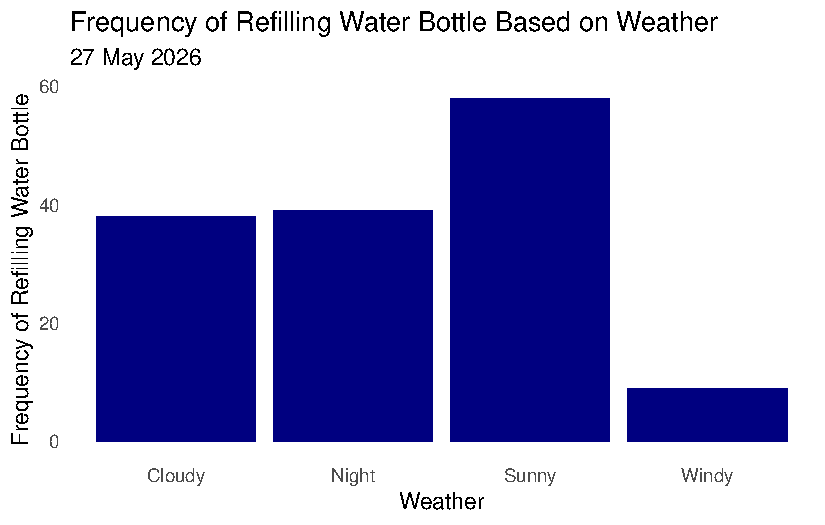
\includegraphics[keepaspectratio]{homework-3_files/figure-pdf/unnamed-chunk-8-1.pdf}}

\begin{Shaded}
\begin{Highlighting}[]
\CommentTok{\#base layer: ggplot}
\FunctionTok{ggplot}\NormalTok{(}\AttributeTok{data =}\NormalTok{ personal\_clean, }
\CommentTok{\#x{-}axis: temperature (Fahrenheit)}
       \AttributeTok{mapping =} \FunctionTok{aes}\NormalTok{(}\AttributeTok{x =}\NormalTok{ temperature\_f)) }\SpecialCharTok{+}
\CommentTok{\#develops a scatterplot for frequency response variables, which can have colors}
  \FunctionTok{geom\_point}\NormalTok{(}\AttributeTok{stat =} \StringTok{"count"}\NormalTok{, }\AttributeTok{color =} \StringTok{"darkred"}\NormalTok{, }\AttributeTok{size =} \DecValTok{1}\NormalTok{) }\SpecialCharTok{+} 
\CommentTok{\#relabel x{-} and y{-}axes, added a subtitle}
  \FunctionTok{labs}\NormalTok{(}\AttributeTok{x =} \StringTok{"Temperature (°F)"}\NormalTok{,}
       \AttributeTok{y =} \StringTok{"Frequency of Refilling Water Bottle"}\NormalTok{,}
       \AttributeTok{subtitle =} \StringTok{"27 May 2026"}\NormalTok{) }\SpecialCharTok{+} 
\CommentTok{\#changed theme from default  }
  \FunctionTok{theme\_minimal}\NormalTok{()}\SpecialCharTok{+}
\CommentTok{\#removed panel background  }
  \FunctionTok{theme}\NormalTok{(}\AttributeTok{panel.background =} \FunctionTok{element\_blank}\NormalTok{()) }\SpecialCharTok{+} 
\CommentTok{\#removed major and minor gridlines   }
  \FunctionTok{theme}\NormalTok{(}\AttributeTok{panel.grid.major =} \FunctionTok{element\_blank}\NormalTok{(),}
        \AttributeTok{panel.grid.minor =} \FunctionTok{element\_blank}\NormalTok{()) }
\end{Highlighting}
\end{Shaded}

\pandocbounded{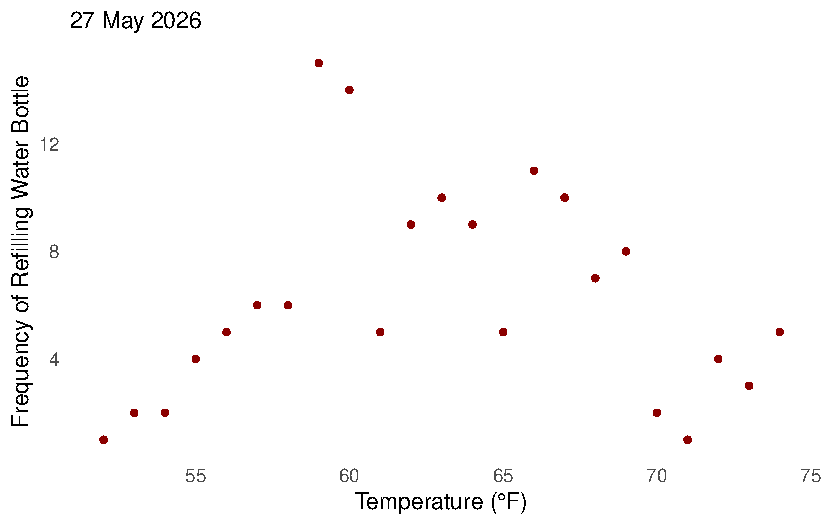
\includegraphics[keepaspectratio]{homework-3_files/figure-pdf/unnamed-chunk-9-1.pdf}}

\subsection{b.}\label{b.-1}

\textbf{Figure 1. Number of times water bottle is refilled depending on
weather.} Each bar (dark blue) represents frequency of water bottle
being refilled every day from weeks 4-9 based on four weather
categories: Cloudy, Night, Sunny, and Windy.

\textbf{Figure 2. Number of times water bottle is refilled based on
temperature.} Points (dark red circles) represent frequency of water
bottle being refilled at a specified temperature every day from weeks
4-9.

\section{Problem 3. Affective
visualization}\label{problem-3.-affective-visualization}

\subsection{a.}\label{a.-2}

For my affective visualization, I want to make it relateable to how
water consumption by humans can negative affect the environment. In
order to do that, I plan to use my bar chart distribution as the
background for how terrestrial life can slowly deteriorate when people
use up water from natural environments. The higher parts of the
distribution can blend into parts of the background that are a lot less
green, symbolism to higher water bottle refill frequency. For my
scatterplot though, I want to use it underwater in my visualization
where every part underneath the highest points in the graph will be
littered with plastic water bottles. The imagery here could be that the
points of highest water bottle refills will have the most plastic water
bottles in my visualization, a symbolism to the litter we have in our
world's waters.

\subsection{b.}\label{b.-2}

\begin{figure}[H]

{\centering \pandocbounded{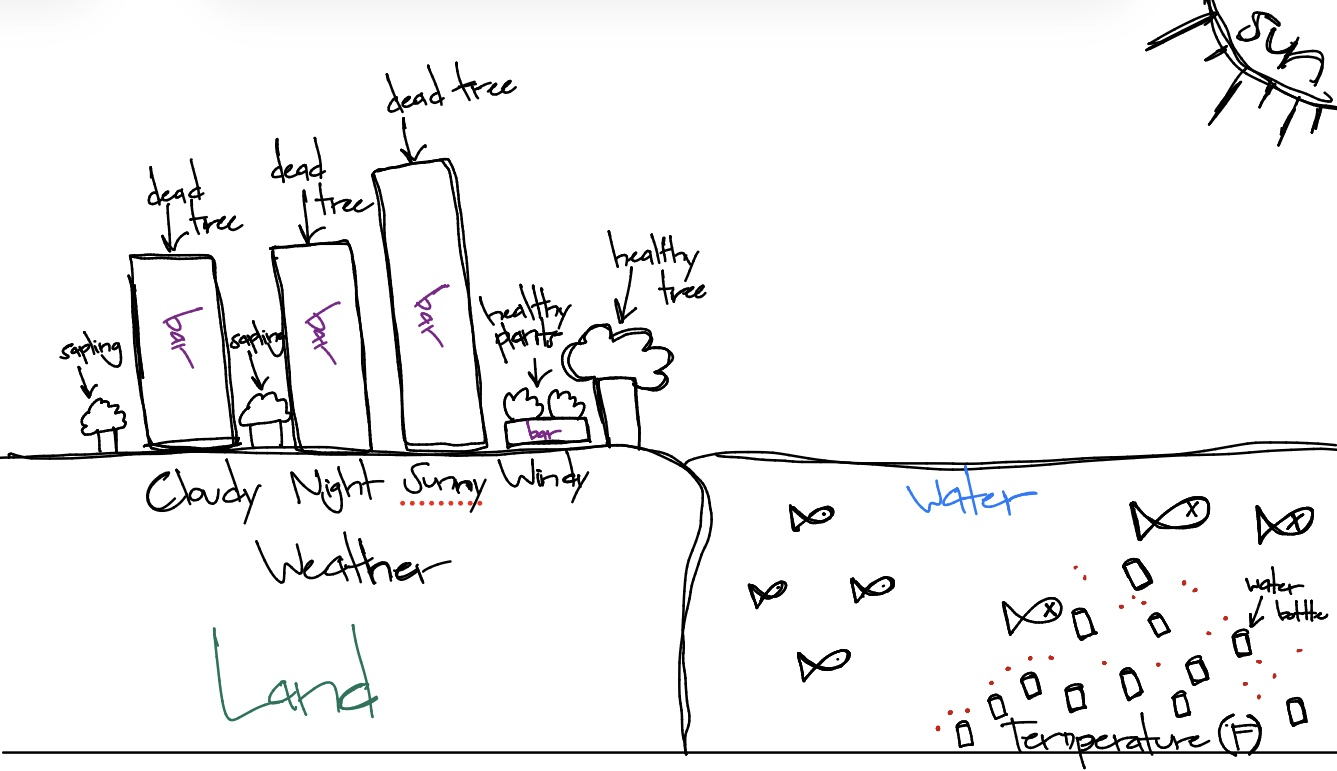
\includegraphics[keepaspectratio]{IMG_0027.png}}

}

\caption{Photo of affective visualization sketch}

\end{figure}%

\subsection{c.}\label{c.-1}

\begin{figure}[H]

{\centering \pandocbounded{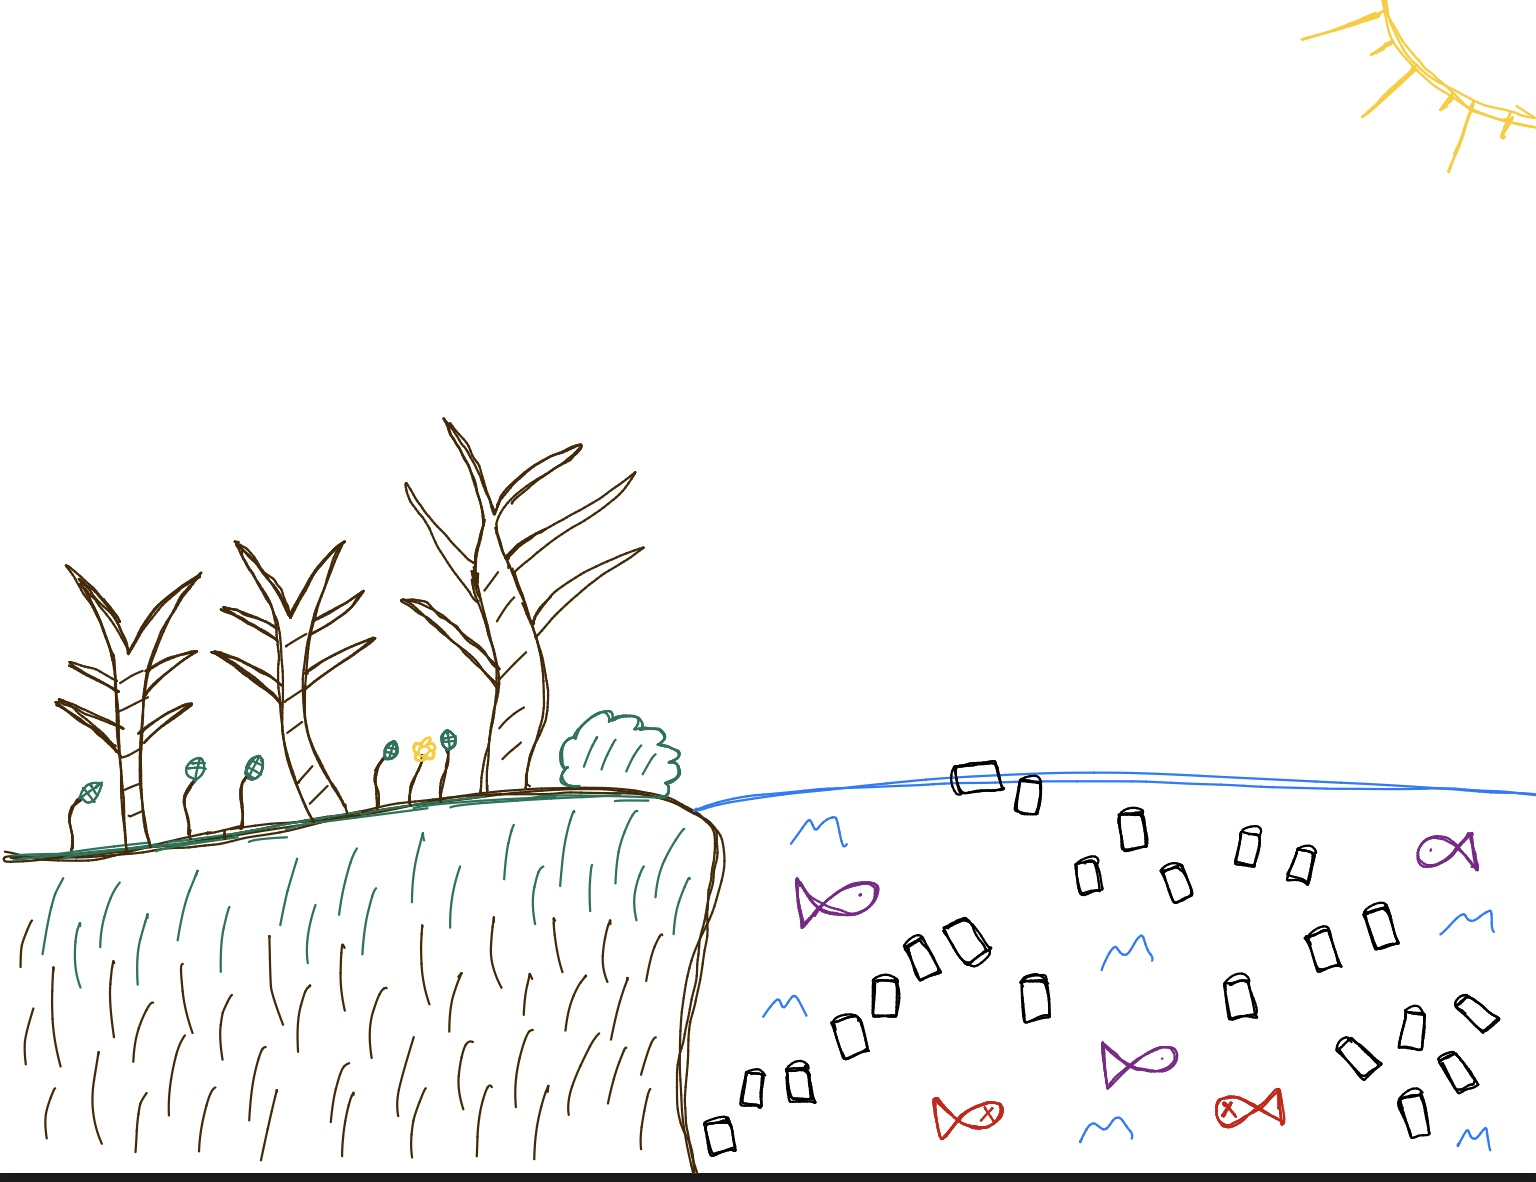
\includegraphics[keepaspectratio]{IMG_0028.png}}

}

\caption{Photo of affective visualization draft}

\end{figure}%

\subsection{d.}\label{d.-1}

For my visualization, I am trying to show the reality of what happens
when we ignore the consequences of protecting the health of the natural
environment through pollution and overharvesting. I would say the main
influence of my piece is just the idea of realism where we document the
the environment as it really is instead of glorifying it as some sort of
separate entity from the urban world. I decided to make my visualization
digitally but drew it out myself, highlighting the two plots I made as
the dead trees represent my bar chart and the plastic bottles flowing in
the water are the points in my scatterplot.

\subsection{e.}\label{e.-1}

\href{https://docs.google.com/presentation/d/1UBWH2dUcW3ISNgImpY5vJY3ra7BDg0eoF2FtFQj7Jqw/edit?slide=id.g3e561da4f6a_0_0\#slide=id.g3e561da4f6a_0_0}{View
Slides}

\section{Problem 4. Statistical
critique}\label{problem-4.-statistical-critique}

\subsection{a.}\label{a.-3}

The name of the test I selected was an analysis of variance (ANOVA). The
response variable is a unit, which is represented by 9 values where 3
are NPS parks in the Sierra Nevadas and the remaining 6 are USFS forests
next to those parks. The predictor variable is the area burned, in
hectares, by prescribed wildfires meant for suppression or resource
benefits.

\begin{figure}[H]

{\centering \pandocbounded{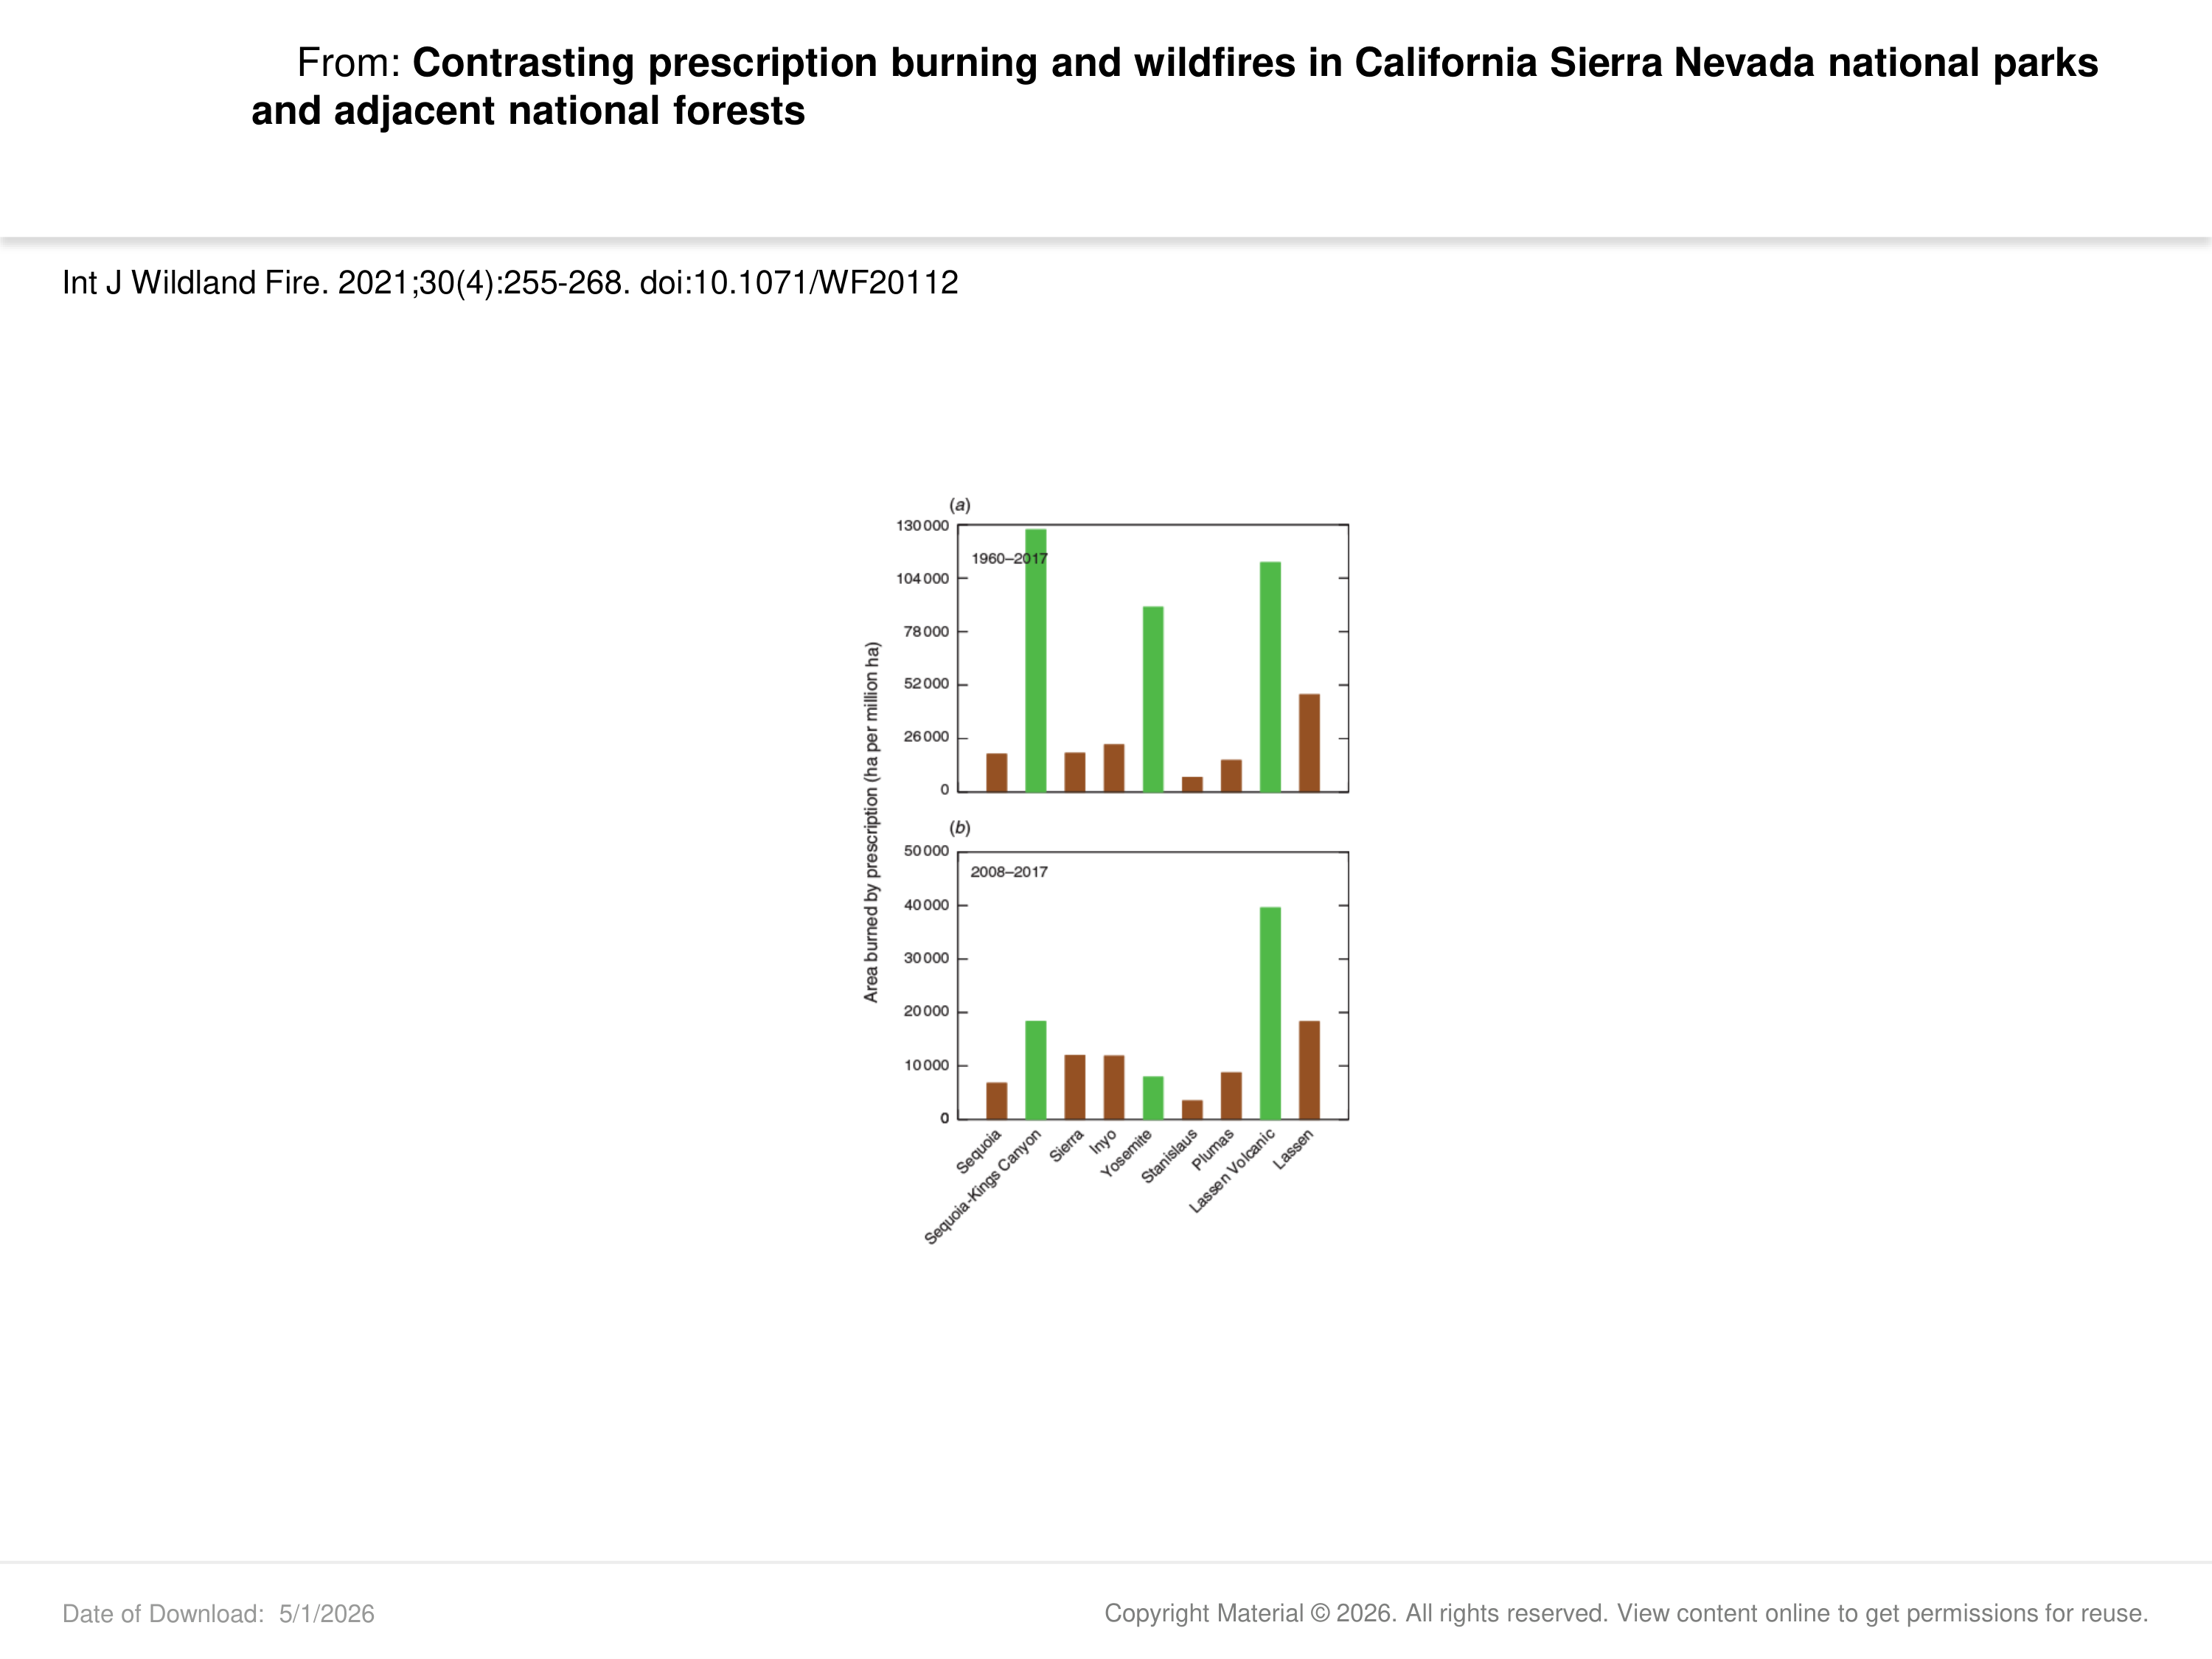
\includegraphics[keepaspectratio]{paper_figure.png}}

}

\caption{Paper figure}

\end{figure}%

\subsection{b.}\label{b.-3}

The authors were relatively clear in visually representing their
statistics in the figures as I could analyze where each bar fell on the
y-axis relative to their label on their x-axis and the colors separated
the type of sites that they looked at. Each of the labels on the x-axis
were long, so they did a really good job in angling it, so each name
could be legible to the reader. However, they did not show any summary
statistics or model predictions.

\subsection{c.}\label{c.-2}

I think the authors only did an okay job at handling the visual clutter
because although they managed to remove the gridlines or most likely
used a minimal theme, the numbers on the y-axis could have been reduced
to an easier unit to read. In addition, the years for when the data was
being recorded literally overlaps with one of the bars in the chart.
Therefore, I would say the data:ink ratio is not very high as there is
lots of wording as well, which is reasonable though since there are 9
bars total in the charts.

\subsection{d.}\label{d.-2}

Something I would change to the figure is to move the years for when the
data was recorded to another part of the figure or even outside of it as
it overlaps with one of the bars, which does not contribute to the
legibility of the figure. Furthermore, I would reduce the units for the
response variable even further so that the numbers on the y-axis would
have less zeros, reducing the about of ink that is on the figure. The
authors may have added the summary statistics or model predictions
separately in another part of the paper, but if that was not the case, I
would probably add that in this case to help us understand any important
values.




\end{document}
